\chapter{NP}

\section{Complexiteit: P en NP}
\begin{figure}[ht]
    \centering
    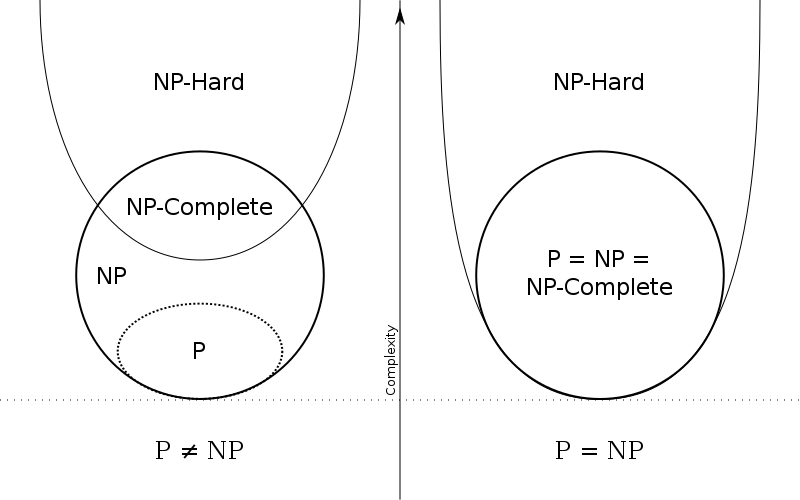
\includegraphics[width=\textwidth]{P_vs_NP}
    \caption{De linkse deelfiguur toont de verschillende complexiteitsklassen indien $P \neq NP$. De rechtse deelfiguur toont hetzelfde indien $P = NP$.}
    \label{fig:P_vs_NP}
\end{figure}

\begin{itemize}
    \item Alle besproken algoritmen hadden een efficiënte oplossing. 
    \item Hun uitvoeringstijd wordt begrensd door een \textbf{veelterm} zoals $O(n^2)$ of $O(n^2m)$.
    \item Sommige problemen hebben hebben geen efficiënte oplossing.
    \item Problemen worden onderverdeeld in \textbf{complexiteitsklassen}.
    \begin{itemize}
        \item Beperking tot  \textbf{beslissingsproblemen}, waarbij de uitvoer \textit{ja} of \textit{nee} is.
        \item Niet echt een beperking omdat elk probleem als een beslissingsproblemen kan geformuleerd worden.
    \end{itemize}
\end{itemize}

\subsection{Complexiteitsklassen}
\begin{itemize}
    \item De klasse \textbf{P} (\textbf{P}olynomiaal) bevat alle problemen waarvan de uitvoeringstijd begrensd wordt door een veelterm.
    \begin{itemize}
        \item Op een realistisch computermodel.
        \begin{itemize}
            \item Heeft een polynomiale bovengrens voor het werk dat in één tijdseenheid kan verricht worden.
        \end{itemize}
        \item Met een redelijke voorstelling van de invoergegevens (geen overbodige informatie, compact, ...).
        \item Al de problemen in \textbf{P} worden als efficiënt oplosbaar beschouwd.
        \alert Waarom een veelterm? $O(n^{100})$ kan nauwelijks efficiënt genoemd worden.
        \begin{enumerate}
            \item Meestal is de graad van de veelterm beperkt tot twee of drie.
            \item Veeltermen vormen de kleinste klasse functies die kunnen gecombineerd worden, en opnieuw een veelterm opleveren.
            \begin{itemize}
                \item Men noemt dit een \textbf{gesloten klasse}.
                \item Efficiënte algoritmen voor eenvoudigere problemen kunnen dus gecombineerd worden tot een efficiënt algoritme voor een complex probleem.
            \end{itemize}
            \item De efficiëntiemaat blijft onafhankelijk van het computermodel.
        \end{enumerate}
    \end{itemize}
    \item De klasse \textbf{NP} (\textbf{N}iet-deterministisch \textbf{P}olynomiaal) bevat alle problemen die door een niet-deterministische computer in polynomiale tijd kunnen opgelost worden en waarvan de oplossing kan gecontroleerd worden in polynomiale tijd.
    \begin{itemize}
        \item Een niet-deterministische computer bevat hypothetisch een oneindig aantal processoren, waarvan er op tijdstap $t$, er $k$ kunnen aangesproken van worden. De processoren werken niet samen, maar kunnen wel hun deel van het probleem oplossen.
        \item Elk probleem uit \textbf{P} behoort tot \textbf{NP}. 
        \item Niet geweten of er probleem in \textbf{NP} zit die niet tot \textbf{P} behoort $\rightarrow \textbf{P}$ vs $\textbf{NP}$ probleem (Figuur \ref{fig:P_vs_NP}). 
        \item Wel geweten dat er problemen zijn die niet in \textbf{NP} zitten, en dus ook niet in \textbf{P}.
    \end{itemize}
    \item De klasse \textbf{NP-hard} bevat alle problemen die minstens even zwaar zijn als elk \textbf{NP}-probleem.
    \begin{itemize}
        \item Een probleem $X$ dat gereduceerd kan worden naar een probleem $Y$ betekent dat $Y$ minstens even zwaar is als $X$.
    \end{itemize}
    \item De klasse \textbf{NP-compleet} bevat alle problemen die \textbf{NP-hard} zijn, maar toch nog in \textbf{NP} zitten.
    \begin{itemize}
        \item Als er één \textbf{NP-compleet} probleem bestaat die efficiënt oplosbaar zou zijn (en dus in \textbf{P} behoort), dan zouden alle problemen uit \textbf{NP} ook efficiënt oplosbaar zijn, zodat $\textbf{P} = \textbf{NP}$.
        \item NP-complete problemen kunnen op verschillende manieren aangepakt worden:
        \begin{itemize}
            \item Backtracking en snoeien.
            \item Speciale gevallen oplossen met efficiënte algoritmen.
            \item Het kan zijn dat de gemiddelde uitvoeringstijd toch goed is.
            \item Gebruik een benaderend algoritme.
            \item Maak gebruik van heuristieken.
        \end{itemize}
    \end{itemize}
    
\end{itemize}

\section{NP-complete problemen}

\begin{itemize}
    \item Overzicht van belangrijke NP-complete (optimalisatie)problemen.
    \item Om na te gaan of een probleem NP-compleet is, moet het herleid kunnen worden naar een basisvorm.
\end{itemize}

\subsection{Het basisprobleem: SAT (en 3SAT)}
\begin{itemize}
    \item Gegeven:
    \begin{itemize}
        \item Een verzameling logische variabelen $\mathcal{X} = \{x_1, \dots, x_{|\mathcal{X}|}\}$.
        \item Een verzameling logische uitspraken $\mathcal{F} = \{f_1, \dots, f_{|\mathcal{F}|}\}$.
        \item Elke uitspraak bestaat uit automaire uitspraken (atomen) samengevoegd met OF-operaties:
        $$f_1 = x_2 \vee \overline{x_5} \vee x_7 \vee x_8$$
    \end{itemize}
    \item Gevraagd:
    \begin{itemize}
        \item  Hoe moeten de waarden toegekend worden aan de variabelen uit $\mathcal{X}$ zodat elke uitspraak in $\mathcal{F}$ waar is?
    \end{itemize}
    \item Elk NP-compleet probleem is reduceerbaar tot SAT.
    \item Een uitspraak met meer dan drie atomen kan herleidt worden naar een reeks uitspraken met elk drie atomen:
    \begin{align*}
        f_1 = &x_2 \vee \overline{x_5} \vee x_n \\
        f_1' = &\overline{x_n} \vee x_7 \vee x_8
    \end{align*}
\end{itemize}

\subsection{Vertex Cover}
\begin{itemize}
    \item Gegegeven:
    \begin{itemize}
        \item Een ongerichte graaf.
    \end{itemize}
    \item Gevraagd:
    \begin{itemize}
        \item Hoe kan de kleinste groep knopen bepaald worden die minsten één eindknoop van elke verbinding bevat.
    \end{itemize}
\end{itemize}